Dos tanques A y B contienen inicialmente 100 litros de salmuera cada uno, con 5 kg de sal
en A y 2 kg en B. Desde \(t=0\), entra agua pura en A a 6 L/min; pasan 8 L/min de A a B,
2 L/min de B a A y salen 6 L/min de B al exterior. La mezcla de cada tanque se mantiene
uniforme. Determinar la cantidad de sal en cada tanque para \(t\ge0\).

\Needspace{4.8cm}
\begin{center}
\begin{minipage}{\linewidth}
\centering
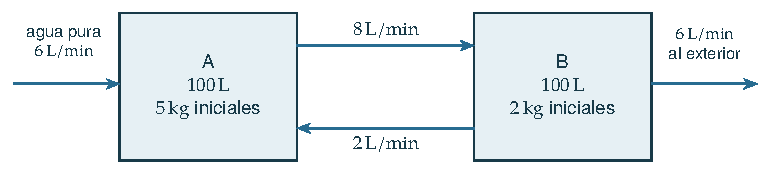
\includegraphics[width=14.62cm]{assets/M2-E0047-setup.pdf}\par
\smallskip{\small Caudales suministrados y cantidades iniciales en los dos tanques.\par}
\end{minipage}
\end{center}
